%%%%%%%% ICML 2026 EXAMPLE LATEX SUBMISSION FILE %%%%%%%%%%%%%%%%%

\documentclass{article}

% Recommended, but optional, packages for figures and better typesetting:
\usepackage{microtype}

\usepackage{graphicx}
\usepackage{subcaption}
\usepackage{booktabs} % for professional tables
\usepackage{bm}
% hyperref makes hyperlinks in the resulting PDF.
% If your build breaks (sometimes temporarily if a hyperlink spans a page)
% please comment out the following usepackage line and replace
% \usepackage{icml2026} with \usepackage[nohyperref]{icml2026} above.
\usepackage{hyperref}


% Attempt to make hyperref and algorithmic work together better:
\newcommand{\theHalgorithm}{\arabic{algorithm}}

% Use the following line for the initial blind version submitted for review:
\usepackage{icml2026}

% For preprint, use
% \usepackage[preprint]{icml2026}

% If accepted, instead use the following line for the camera-ready submission:
% \usepackage[accepted]{icml2026}

\usepackage{amsmath}
\usepackage{amssymb}
\usepackage{mathtools}
\usepackage{amsthm}


% if you use cleveref..
\usepackage[capitalize,noabbrev]{cleveref}

%%%%%%%%%%%%%%%%%%%%%%%%%%%%%%%%
% THEOREMS
%%%%%%%%%%%%%%%%%%%%%%%%%%%%%%%%
\theoremstyle{plain}
\newtheorem{theorem}{Theorem}[section]
\newtheorem{proposition}[theorem]{Proposition}
\newtheorem{lemma}[theorem]{Lemma}
\newtheorem{corollary}[theorem]{Corollary}
\theoremstyle{definition}
\newtheorem{definition}[theorem]{Definition}
\newtheorem{assumption}[theorem]{Assumption}
\theoremstyle{remark}
\newtheorem{remark}[theorem]{Remark}

% Todonotes is useful during development; simply uncomment the next line
%    and comment out the line below the next line to turn off comments
% \usepackage[disable,textsize=tiny]{todonotes}
\usepackage[textsize=tiny]{todonotes}

% The \icmltitle you define below is probably too long as a header.
% Therefore, a short form for the running title is supplied here:
\icmltitlerunning{Bellman-Smoothed Regression for Value Function Estimation}

\begin{document}

\twocolumn[
  \icmltitle{Bellman-Smoothed Regression for Value Function Estimation}

  % It is OKAY to include author information, even for blind submissions: the
  % style file will automatically remove it for you unless you've provided
  % the [accepted] option to the icml2026 package.

  % List of affiliations: The first argument should be a (short) identifier you
  % will use later to specify author affiliations Academic affiliations
  % should list Department, University, City, Region, Country Industry
  % affiliations should list Company, City, Region, Country

  % You can specify symbols, otherwise they are numbered in order. Ideally, you
  % should not use this facility. Affiliations will be numbered in order of
  % appearance and this is the preferred way.
  \icmlsetsymbol{equal}{*}

  \begin{icmlauthorlist}
    \icmlauthor{Dillon Sandhu}{sch}
    \icmlauthor{Ronald Parr}{sch}
  \end{icmlauthorlist}


  \icmlaffiliation{sch}{Department of Computer Science, Duke University, Durham, North Carolina, USA}

  \icmlcorrespondingauthor{Dillon Sandhu}{dillon.sandhu@duke.edu}
  \icmlcorrespondingauthor{Ronald Parr}{parr.cs@duke.edu}

  % You may provide any keywords that you find helpful for describing your
  % paper; these are used to populate the "keywords" metadata in the PDF but
  % will not be shown in the document
  \icmlkeywords{Reinforcement Learning}

  \vskip 0.3in
]

% this must go after the closing bracket ] following \twocolumn[ ...

% This command actually creates the footnote in the first column listing the
% affiliations and the copyright notice. The command takes one argument, which
% is text to display at the start of the footnote. The \icmlEqualContribution
% command is standard text for equal contribution. Remove it (just {}) if you
% do not need this facility.

% Use ONE of the following lines. DO NOT remove the command.
% If you have no special notice, KEEP empty braces:
\printAffiliationsAndNotice{}  % no special notice (required even if empty)
% Or, if applicable, use the standard equal contribution text:
% \printAffiliationsAndNotice{\icmlEqualContribution}

\begin{abstract}
  Value function estimation is a core problem in Reinforcement Learning.
  Monte-Carlo methods compute an unbiased estimate of the value function, but can suffer variance 
  related to the length and noisiness of the task.
  Temporal differences methods (TD Learning) are popular in part because they reduce variance, and in part because they induce local Bellman-consistency of the learned value function. 
  However, TD learning can fail to converge when using non-linear function approximation.
  We study a new learning rule based on the minimization of a convex Bellman-smoothed value loss.
  We extend previous results that show when TD learning succeeds at lowering the Bellman-smoothed value loss. 
  Our main contribution is using this loss for value function learning in deep RL. 
  We first show how to estimate the new objective in an unbiased fashion from trajectory data -- with strictly lower variance than Monte Carlo.
  We show that in expectation, the learned value function leads to stronger policy improvement than classical TD learning.
  We experiment on RL tasks, including continuous control, showing that our value function loss improves the performance of PPO.
\end{abstract}

\section{Introduction}
\section{Preliminaries}
\begin{align}
  D &\doteq \text{diag}(\bm{\mu}) \label{def:D} \\
  A &\doteq D(I-\gamma P) \label{def:A}
\end{align}

If the Bellman Operator is a contraction in the $D$-weighted norm, then $A$ is positive definite \cite{Tsitsiklis1997Analysis}. We make use of the labels $S$ and $K$ for its symmetric and skew symmetric components respectively.
\begin{align}
  A &= \frac{1}{2} (A + A^\intercal) + \frac{1}{2}(A - A^\intercal) \\
    &= S + K \label{def:SK}
\end{align}

The objective is to train a differentiable value estimate $v_\theta$, with $|\theta|=k$.  
The estimated value vector $\bm{v}$ is defined by stacking each state's value prediction, so that $\bm{v}(i) = v_\theta(s_i)$. The value error vector is given by
\begin{align}
  \bm{e} \doteq (\bm{V}-\bm{v}).
\end{align}

The fundamental goal of policy evaluation is to improve the policy. The instrumental goal is to minimize the following error, called the MSE. 
\begin{equation}
  \mathcal{L}_{MC} \doteq \|\bm{e}\|_D^2. \label{eq:mc_loss}
\end{equation}

In expectation, Monte Carlo value learning minimizes \ref{eq:mc_loss}, with errors estimated in an unbiased fashion from sampled episodes. In contrast, bootstrapping methods like Temporal Difference (TD) Learning \cite{sutton_td} instead use the notion of the Bellman (or TD) error, given by:
\begin{equation}
  \bm{\delta} = \bm{R} + \gamma P \bm{v} - \bm{v}. \label{eq:td_error}
\end{equation}
TD learning is an iterative algorithm that is based on relationship between the Bellman error and the gradient of the value estimator. We will write its expected update in matrix form, stacking the gradients at each state into the $N \times k$ Jacobian matrix, $J_\theta$: 
\begin{align}
  J_\theta
  &\doteq
  \begin{bmatrix}
    \nabla v_\theta(s_1)^\top \\
    \nabla v_\theta(s_2)^\top \\
    \vdots \\
    \nabla v_\theta(s_N)^\top
  \end{bmatrix}
  \in \mathbb{R}^{N \times k}.
\end{align}
In expectation, the TD update and loss are given by the following two equations.
\begin{align}
\bm{\theta} &\xleftarrow{TD} \bm{\theta} + \alpha  J_\theta^\intercal D \bm{\delta} \label{eq:td_update_expected} \\
\mathcal{L}_{TD} &\doteq  \|\bm{R} + P\overline{ \bm{v} } - \bm{v}\|_D^2 
\end{align}
Where $\overline{f_\theta}$ indicates the stop gradient operator is applied to $\theta$. A \textit{TD Fixed Point} is a value of $\theta$ where no update occurs in expectation. A TD fixed point is reached whenever $\bm{0}_k = J_\theta^\intercal D \bm{\delta} =\mathbb{E}_{s \sim \mu} (\delta(s) \nabla v(s))$. 

It is known \cite{Tsitsiklis1997Analysis} that \eqref{eq:td_update_expected} can be rewritten using the substitution $A \bm{e} = D(I-\gamma P)(\bm{V}-\bm{v}) = D(\bm{R}-(I-\gamma P)\bm{v} = D \bm{\delta}$. This substitution is a key insight from \citep{tang2023towards}'s analysis of deep TD learning, and means \eqref{eq:td_update_expected} can be rewritten as:
\begin{equation}
  \bm{\theta} \xleftarrow{TD} \bm{\theta} + \alpha  J_\theta^\intercal A \bm{e}
  \label{eq:td_update_expected_A}
\end{equation}

\section{Related Work}
[TODO]
\section{Policy Optimization Bellman-Smoothed Value Error}
The Bellman-Smoothed value error from \cite{tang2023towards} is given by:
\begin{equation}
  E \doteq  \|\bm{V} - \bm{v}\|_S^2 = \bm{e}^\intercal A \bm{e} = \bm{e}^\intercal S \bm{e}. \label{eq:E}
\end{equation}
Since $S$ is positive definite, $E \geq 0$, with equality when the value error is zero at all states where $\bm{\mu}(s) >0$. We study gradient descent on $E$, which makes the following update:
\begin{align}
  \bm{\theta} &\xleftarrow{E} \bm{\theta} + \alpha  J_\theta^\intercal S \bm{e} \label{eq:E_update_expected} 
\end{align}
\begin{proposition} \label{prop:td_vs_E_update}
  The expected update due to gradient descent on $E$ is equal to the expected update due to TD learning, less $J_\theta^\intercal K \bm{e}$, where $K = \frac{1}{2}(A - A^\intercal)$ is the skew-symmetric component of $A$.
\end{proposition}
\begin{proof}
  \begin{align}
    J_\theta^\intercal S \bm{e} =  J_\theta^\intercal (A-K) \bm{e} = J_\theta^\intercal A\bm{e} - J_\theta^\intercal K \bm{e}
  \end{align}
\end{proof}

Since the Bellman-Smoothed Value Error is the $S$-weighted norm of the value error vector, $E$ can be treated as a squared error. It is convex in $\bm{v}$, and minimized when the value error is zero at all visited states. Under typical assumptions gradient descent can be shown to converge to a local minimum of $E$ (as in supervised learning). In contrast, exact TD learning may not converge. Moreover, its fixed points may have positive value error \cite{Tsitsiklis1997Analysis}. This is due to the skew-symmetric component $K$ in the TD update. A TD fixed point can have non-zero value error if $J_\theta^\intercal S \bm{e} = - J_\theta^\intercal K \bm{e}$.  The presence of $K$ also implies that the $TD$-Learning update \eqref{eq:td_update_expected_A} can increase the value error $E$, possibly leading to divergence [TODO: prove]. \citep{tang2023towards} showed that when the Markov Chain is reversible ($DP = (DP)^\intercal$), TD learning is equivalent to gradient descent on $E$.\footnote{In the reversible case $A$ is symmetric and $\bm{e}^\intercal K \bm{e}$ equals zero.} However, in practical RL, the MDP is rarely reversible.

Despite these theoretical limitations, on-policy TD learning is popular. For one, the sampled update (e.g. the Monte Carlo estimator of \eqref{eq:td_update_expected}) has low variance due to only incorporating one-step noise. Secondly, with tabular and linear function approximators, the TD-fixed point and the model-based solution are the same -- a fact known as the certainty equivalence principle (\citep{sutton_td}, \citep{parr2008analysis}). Third, TD-learning ascribes similar values to neighboring states, while Monte Carlo treats each state as disconnected. 

As discussed later, $E$-minimization smooths the value function in a similar manner to TD learning, while remaining a safer optimization target. In the next section, we present empirical evidence that the exact version of E minimization compares favorably to exact TD and exact MC. Additionally, we present a form of $E$ that can be sampled, with variance lying exactly between that of TD and MC.

\textbf{Experiment: Comparing Expected Versions of the Algorithms}
We find empirically that TD learning performs worse than $E$ minimzation when the Markov Chain has a significant skew-symmetric component. We study the behavior of $E$ and $\mathcal{L}_{TD}$ and on nine environments, which are small enough to solve exactly.

\begin{itemize}
  \item \textbf{Four Rooms (Sparse)}: 104 states (105 including terminal). A classic sparse reward navigation task on a $13 \times 13$ grid with 104 traversable cells partitioned into four rooms. The state representation is a grid, and a CNN is used for the value network.
  \item \textbf{Four Rooms + Mines (Sparse and Dense)}: Adds mines which terminate the agent's life. Dense versions of navigation tasks use potential-based reward shaping based on distance to the goal.
  \item \textbf{Eight Rooms (Sparse and Dense)}: 210 states (211 including terminal). An extended navigation task on a $25 \times 13$ grid with eight rooms.
  \item \textbf{Mountain Car (Sparse and Dense)}: A continuous state space (discreteized for tabular solvers). Dense rewards are obtained with potential (height)-based reward shaping.
  \item \textbf{Space Invaders}: 1,974 states (1,975 including terminal). A tabular 3-alien shielded-fleet version of Space Invaders on a $7 \times 6$ grid, with endless waves and termination only on death.
  \item \textbf{Whirlpool}: 105 states (105 including terminal). A gridworld using the same visual state representation as Four Rooms. The agent starts in the outermost part of the grid, and must navigate to the center of the whirlpool. A strong force pushes the agent clockwise, in the sense that the agent's action succeeds only 10\% of the time, and 90\% of the time the agent is pushed clockwise.
\end{itemize}
As we shall see, Whirlpool, Space Invaders, and Mountain Car all have strong skew-symmetry. Informally, these MDPs are far from reversible. A reversible MDP has the same probability flow transitioning ``forward'' from $s \rightarrow s'$ as it does transitioning ``backward'' from $s' \rightarrow s$. In skew-symmetric MDPs, either the dynamics move only forward, or a strong asymmetric force acts on the agent (e.g. gravity in Mountain Car).

The above environments are small enough that we can exactly compute the TD update \eqref{eq:td_update_expected}, the MSE loss \eqref{eq:mc_loss}, and Bellman-Smoothed Value Error \eqref{eq:E}. This removes any noise in the updates. We use deep value function approximation, using a CNN on visual tasks and a MLP on Mountain Car. The only randomness across runs is from neural network initialization. Hyperparamters can be found in the Appendix [TODO: put in hypers].
% e train a policy with PPO \cite{schulman2017proximal}, and then, holding it fixed, train a neural network. 
We first consider fixed policy evaluation. For each algorithm, we train a neural network to estimate the value of the uniform random policy. We denote the size of the final hidden layer by $k$, and try $k=8$ and $k=64$ to understand the impact of the capacity of the network. Since the Markov Chain is fixed, we can compute its skew-symmetry as the ratio of $\|K\|$ to $\|S\|$. For a reversible Markov Chain, $\|K\|$ will be zero. We plot this skew-symmetry measure against the relative error -- the average MSE during learning for $E$ relative to $TD$. A lower relative error means $E$ performed better. Note that we use the on-policy MSE, which is the typical objective in policy evaluation, though neither algorithm minimizes it directly.

Figure \ref{fig:alignment_vs_skew_symmetry} shows that, as Proposition \ref{prop:td_vs_E_update} suggests, when $K$ is small compared to $S$, $E$ minimization and $TD$ have the same MSE during learning. This is because their learning dynamics are almost the same, as Proposition \ref{prop:td_vs_E_update} suggests. However, as the environment becomes more skew-symmetric, TD learning's performance declines relative to $E$ minimization.

% ----------------------------------------------------------------
% Figure: Alignment
% ----------------------------------------------------------------
\begin{figure*}[tbp]
  \centering
  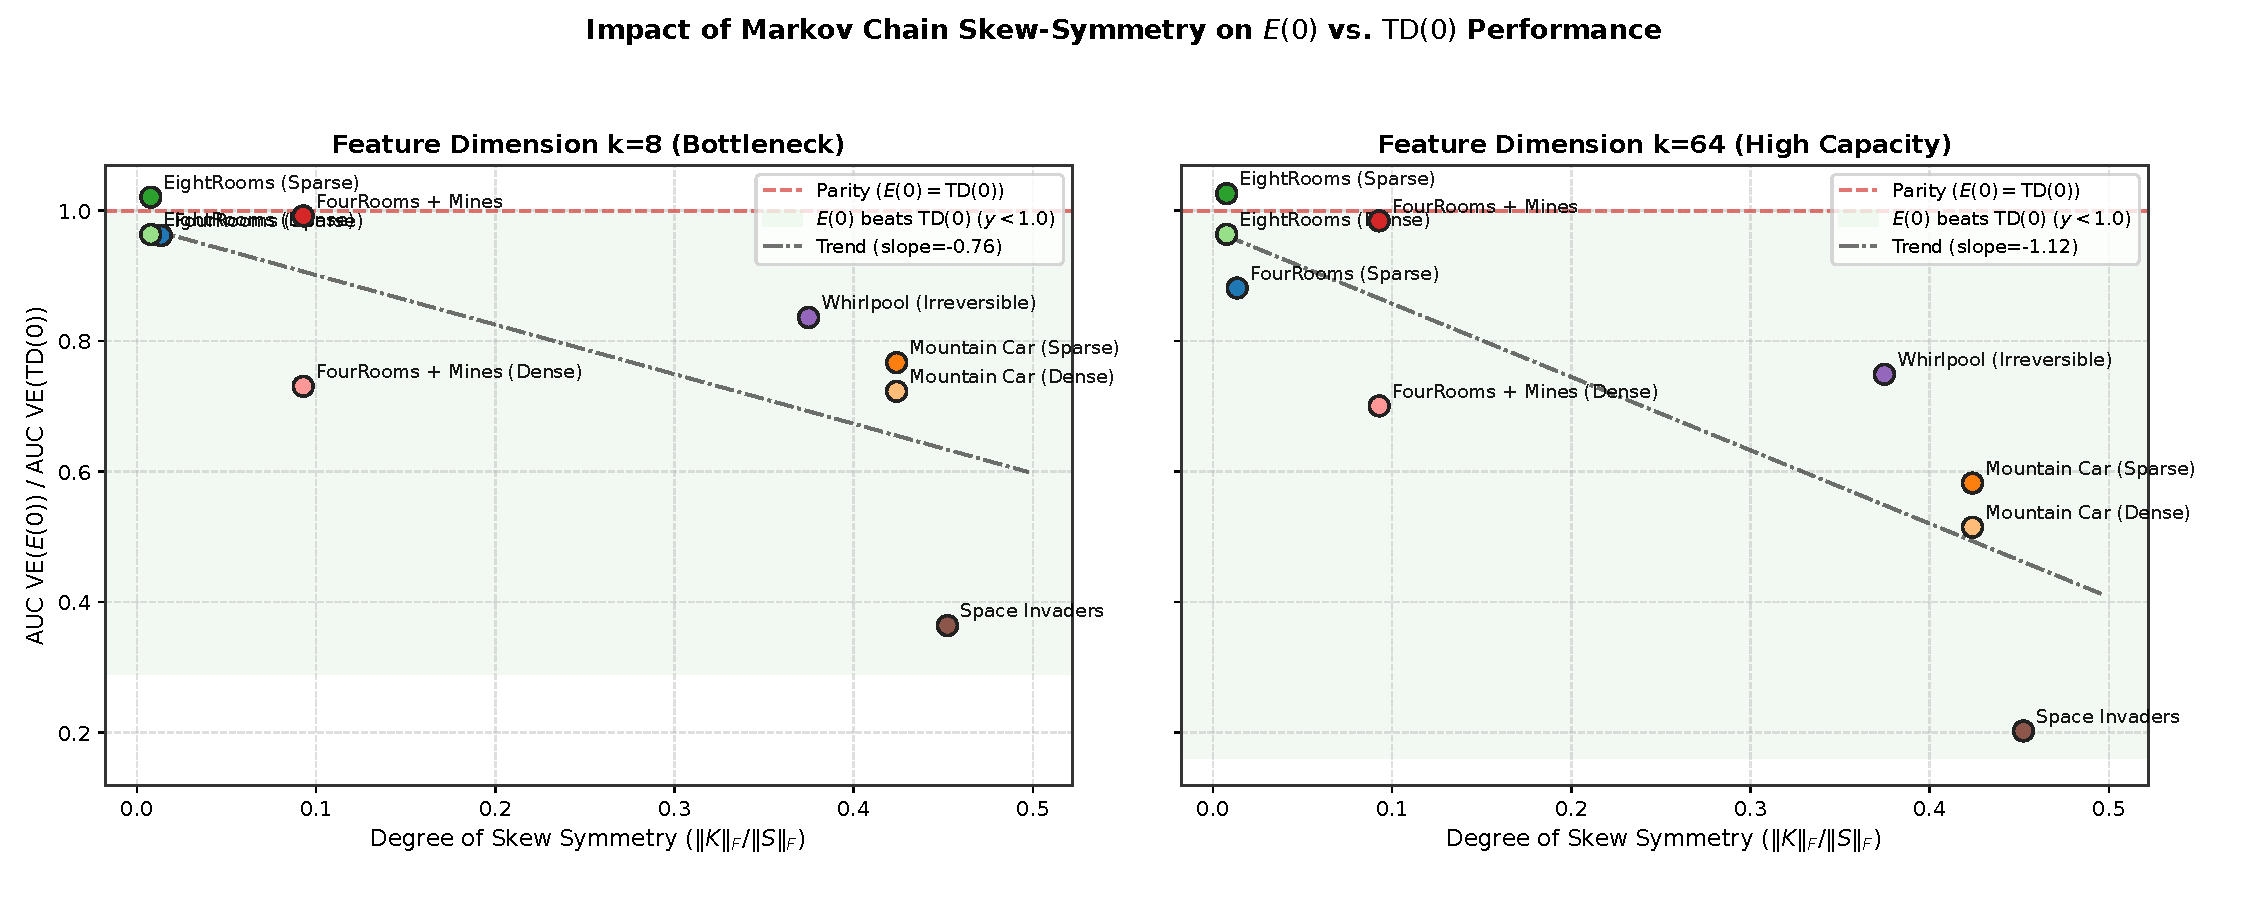
\includegraphics[width=\textwidth]{figures/skew_symmetry_vs_e0_td0_scatter.pdf}
  \caption{\textbf{Alignmnent vs. Skew Symmetry}  Environments charted by their alignment based on the ratio of the norm of $K$ to the norm of $S$ and the relative performance of exact TD vs. exact E-Minimization $\frac{\text{AUC}(MSE_E)}{\text{AUC}(MSE_{TD})}$. The negative slope captures the fact that in more skew-symmetric environments, $E$ has better value learning. 10 seeds.}
  \label{fig:alignment_vs_skew_symmetry}
\end{figure*}
% ----------------------------------------------------------------
% End Figure
% ----------------------------------------------------------------

While the MSE is the de-facto objective for fixed policy evaluation, the goal of policy evaluation is policy improvement. We run the three algorithms to evaluate the uniform random policy. In addition to TD and $E$-minimzation, we also consider \textbf{Exact Monte Carlo} (MC), which is the minimzation of $\mathcal{L}_{MC}$ directly by fitting the true value function in a supervised fashion. Despite the name ``Monte Carlo'', the exact MC update has no noise besides random neural network initialization.

\begin{table*}[tbp]
  \centering
  \begin{tabular}{lrrrrr}
  \toprule
  \textbf{Algorithm} & \textbf{MSE (AUC)} & \textbf{MSE (Final)} & \textbf{Advantage Acc.} & \textbf{Value of Greedy Policy} \\
  \midrule
  TD & (0.0/9) [0w+0t] & (0.3/9) [0w+1t] & (0.0/9) [0w+0t] &  (2.0/9) [2w+0t]  \\
  MSE Minimization & \textbf{ (4.5/9) [4w+1t]} & \textbf{ (7.3/9) [7w+1t]} &  (3.0/9) [2w+2t] &  (3.0/9) [2w+2t] \\
  E Minimization & \textbf{ (4.5/9) [4w+1t]} &  (1.3/9) [1w+1t] & \textbf{ (6.0/9) [5w+2t]} & \textbf{ (4.0/9) [3w+2t]} \\
  \bottomrule
  \end{tabular}
  \caption{Win Rate of TD, MC, and E minimization across several metrics: The AUC and final MSE as well as two measures of policy improvement: (1) the cosine similarity between the learned and true advantage functions, and (2) the value of the greedy policy at the start staet. For each environment, an algorithm is a winner if it performs best on a certain metric. Ties occur when no single algorithm was statistically significantly best, and are split evenly. Thus $1.5/9$ indicates that the algorithm won outright on exactly one environment and tied on another.}   \label{tab:table4_env_win_rate_triad_k64}
  \end{table*}
  
  Results are shown in \ref{tab:table4_env_win_rate_triad_k64}. Exact MC usually obtains the best MSE by the end of learning, which makes sense as the MSE is its learning objective. We note that $E$-minimization learns the value function quickly -- as measured by the training AUC of the MSE. We also consider two metrics designed to inform us of the quality of the learned value function for the purposes of policy improvement. Metric one is the start-state value of the greedy policy on the learned value function. This is the average return that would be obtained following the geredy policy. Metric one measures the strength of the policy due to a single round of approximate policy iteration. Metric two measures the quality of the policy gradient: the policy gradient can be shifted or scaled by a constant without affecting the policy update. As such, we measure the cosine-similarity, or normalized dot product, of estimated advantage and true advantage (the advantage is tread as a vector in state-action space). Since we learn value functions, we compute the estimated advantage as $\bm{a} =\bm{R} + \gamma P \bm{V}$. We observe that by both of these metrics, exact $E$-minimization learns a value function that is better for policy improvement.

  \begin{figure*}[tbp]
    \centering
    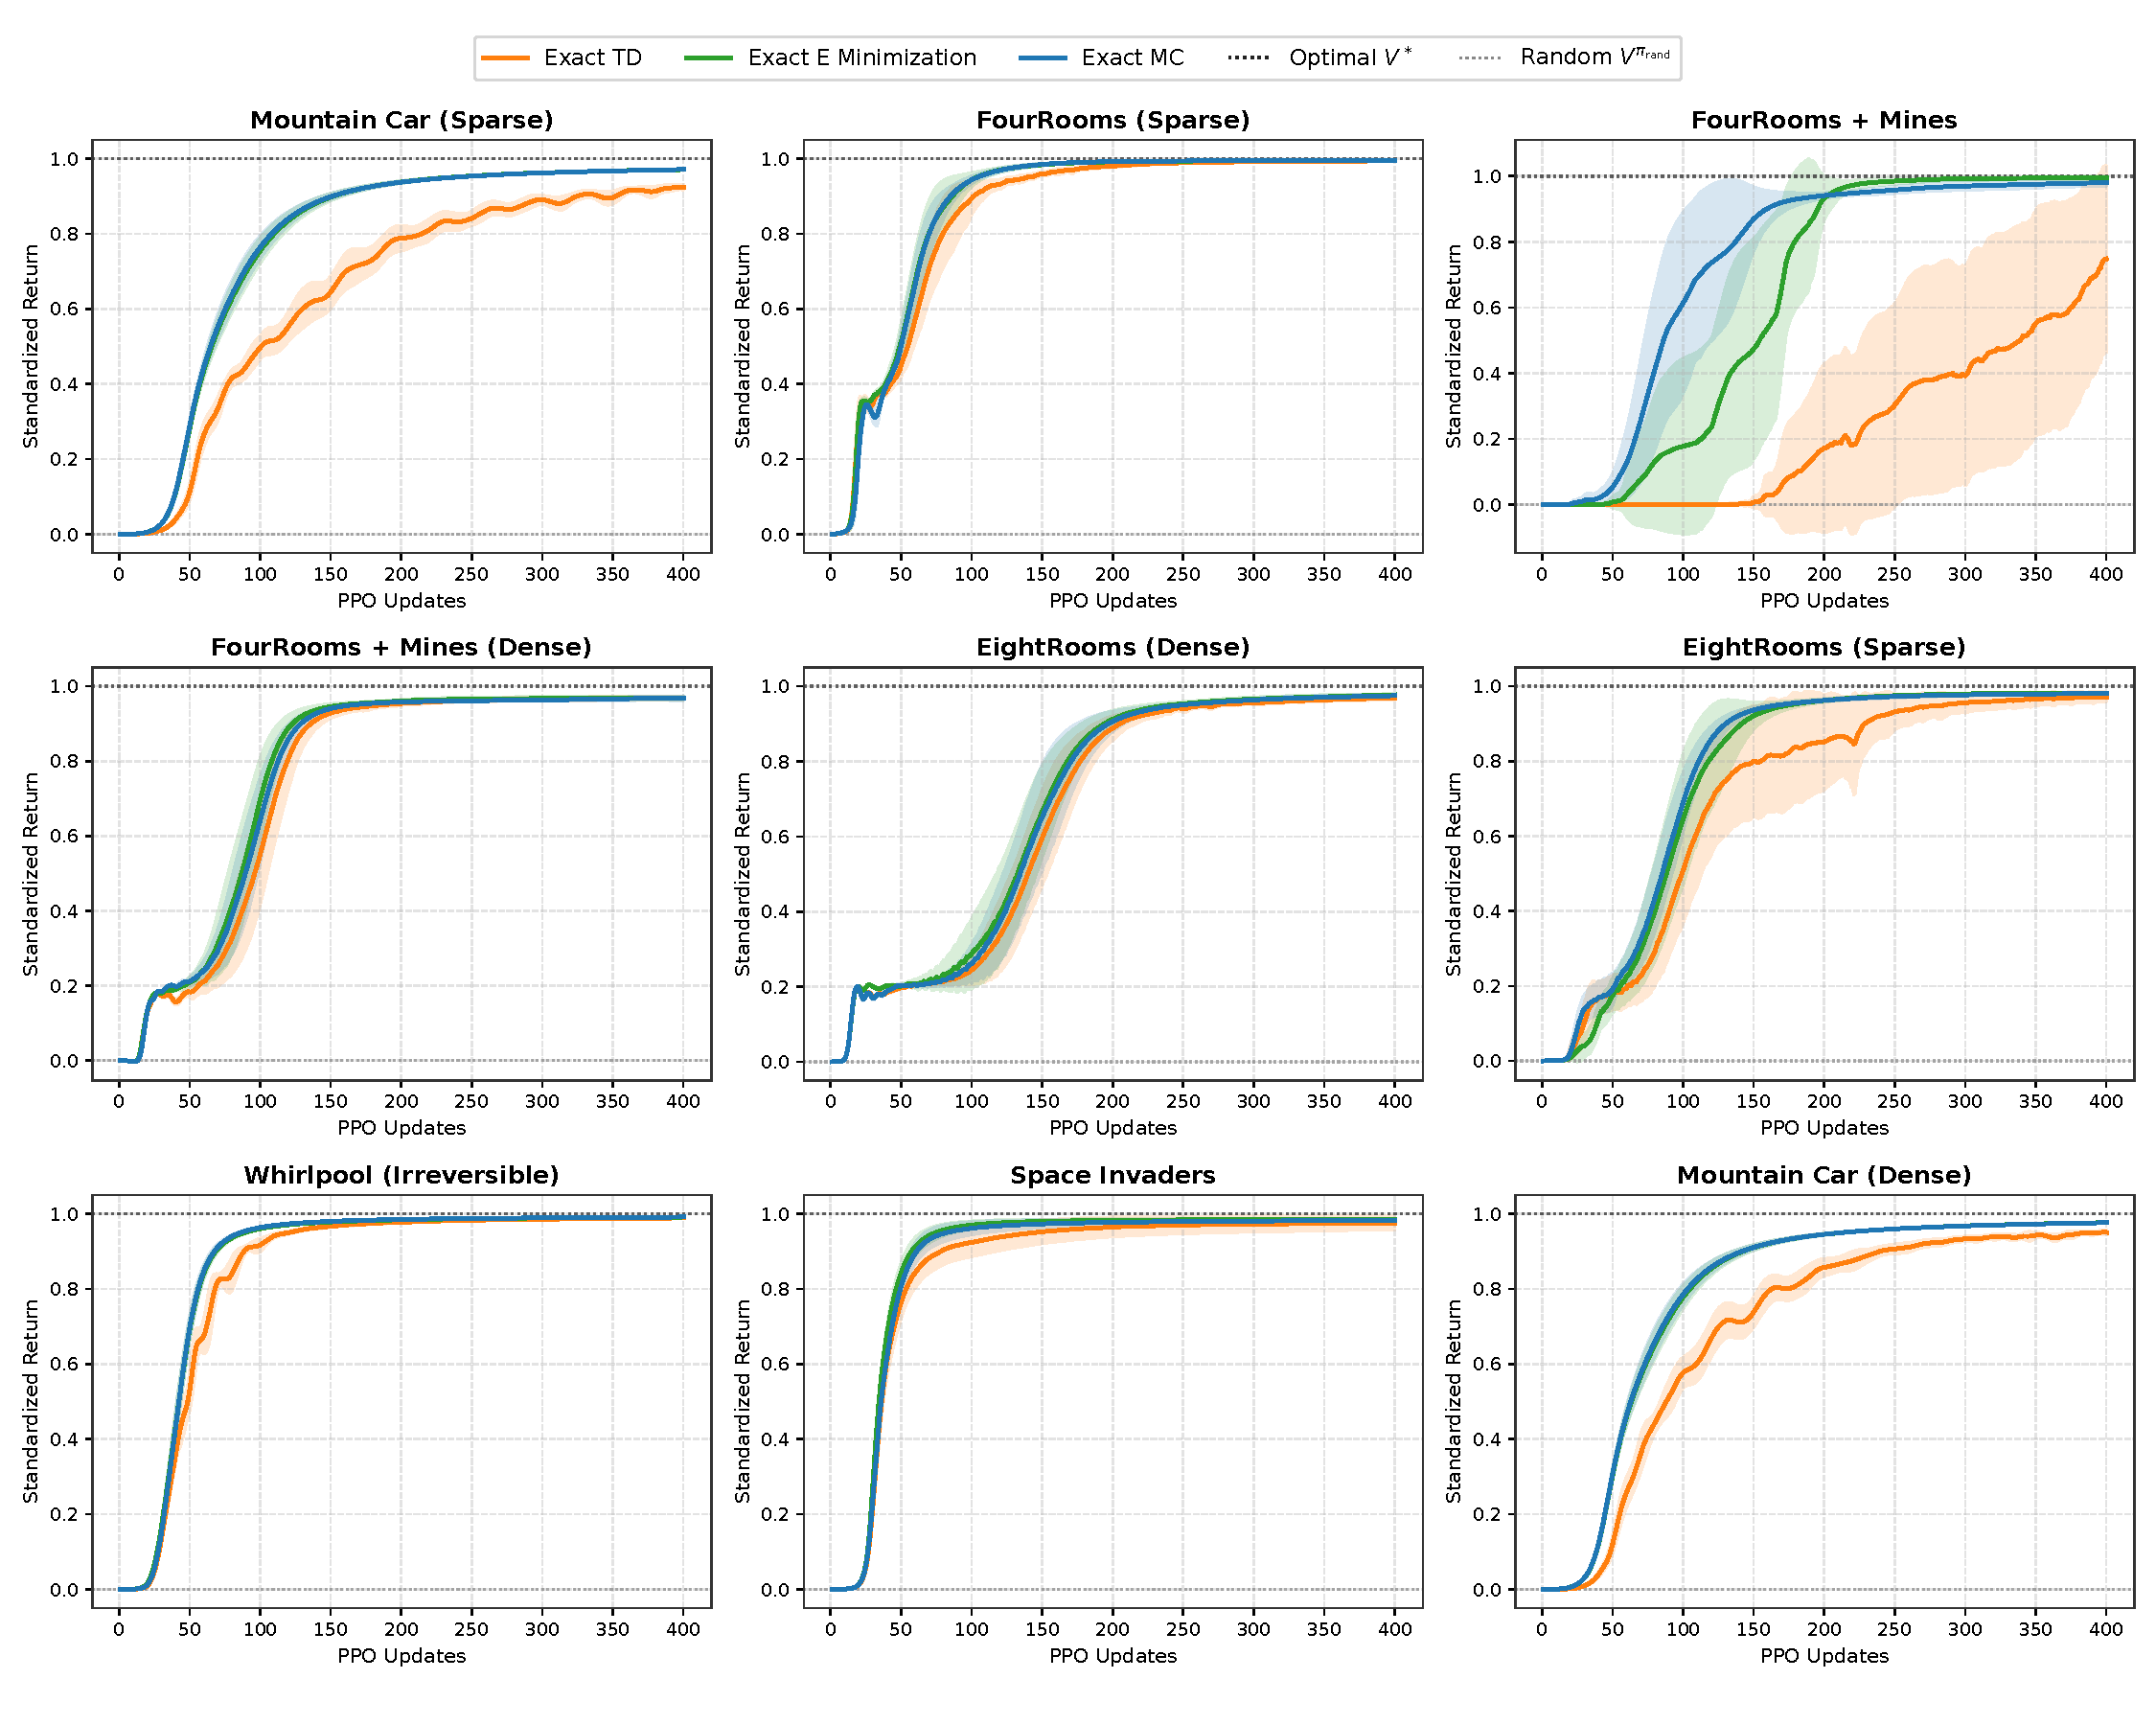
\includegraphics[width=\textwidth]{figures/standardized_performance_learning_curves.pdf}
    \caption{\textbf{Exact PPO.} Learning curves for no-sampling PPO with the critic due to exact TD, MC, or $E$-minimization. 10 seeds.}
    \label{fig:exact_ppo}
  \end{figure*}

  \textbf{Expected PPO.} To see if these results carry over to policy optimization, we implement a no-sampling version of PPO, with a critic is due to exact E, exact TD, or exact MC. The policy is paramterized by an actor network with the same architecture as the critic, without parameter sharing between actor and critic. We use a constant learning rate for the actor, but tune the critic learning rate for each algorithm. Results for the best tuned setting are shown in Figure \ref{fig:exact_ppo}. Unlike the fixed policy evaluation task, PPO updates both the actor and critic at each round. This means that the learning algorithm must be able to evaluate a new policy quickly, with transfer between policies. We see that TD learning struggles with sparse rewards (see EightRooms Sparse and Dense), possibly because it would require more iterations to propagate value through the state space. However, TD also struggles with dense, skew-symmetric tasks like Dense Mountain Car and Space Invaders.


\section{Sampling the Bellman-Smoothed Value Error}
\begin{theorem} \label{thm:sampledE}
  If $\bm{\mu}$ is the stationary distribution ($\bm{\mu}^\intercal P = \bm{\mu}$), the Bellman-Smoothed Value Error can be written as
\begin{align}
  E &= (1-\gamma) \|\bm{e}\|_D^2 + \gamma \mathcal{E},
\end{align}
where the energy, $\mathcal{E}$, is given by the following.
\begin{align}
  \mathcal{E}
  &= \frac{1}{2} \sum_{ij}\mu_i p_{ij}
  (e_i - e_j)^2 \label{def:energy} \nonumber
  \\
  &= \frac{1}{2} \sum_{ij}\mu_i p_{ij}
  (\underbrace{r_i + \gamma v(s_j) - v(s_i)}_{=\hat{\delta}_i}
    + (1-\gamma)e_j)^2 \label{eq:energytdform}
\end{align}
\end{theorem}

Equation \ref{eq:energytdform} emphasizes that the energy $\mathcal{E}$ is the sum of
squared terms, each of which can be estimated on-policy. 
Each squared term is the sum of the sampled TD error and \textit{next state} Monte-Carlo error. Notice that the total weight on Monte-Carlo terms is $O((1-\gamma)^{-1})$, reducing their variance.


\begin{proposition}
The Bellman-Smoothed Value Error is equal to the 
$D$-weighted inner product of the value error and the TD-error.
\begin{align}
  E = \bm{e}^\intercal D \bm{\delta}
\end{align}
\end{proposition}

\begin{corollary}
  The magnitude of $E$ is bounded by the magnitude of the Monte-Carlo and TD losses.
  \begin{align}
  E = \langle \bm{e}, \bm{\delta} \rangle_D \le \|\bm{e}\|_D \|\bm{\delta}\|_D
  \end{align}
\end{corollary}

One can obtain an unbiased sample of $e_i$ using the empirical return $G_i \doteq \sum_{t\geq 0} \gamma^t r_t$.

\textbf{Gradient of the Energy}
Recall that $\bm{e}$ depends on $\theta$, with $\nabla_\theta \bm{e} = -\nabla_\theta v_\theta$. The gradient of the energy can be written as the sum of many terms, weighted by the frequency under $\bm{\mu}$:
  \begin{align}
  \nabla_\theta \mathcal{E} &=  \mu_i \underbrace{\nabla_\theta \frac{1}{2}\sum_{i} \sum_jp_{ij}
  (e_i - e_j)^2}_{\nabla_\theta \mathcal{E}_i}  \nonumber 
  \end{align}
Further examining each of these terms:
\begin{align}
   \nabla_\theta \mathcal{E}_i  &=  \frac{1}{2} \sum_jp_{ij} \nabla_\theta(e_i - e_j)^2 \\
   &=   \sum_jp_{ij}
  (e_i - e_j)\nabla_\theta(e_i - e_j) \\
    &=    \sum_jp_{ij}
  (e_i - e_j) (\nabla_\theta v_\theta(s_j) -\nabla_\theta v_\theta(s_i)) \\
      &=    \underbrace{\sum_jp_{ij}
  (e_i - e_j) \nabla_\theta v_\theta(s_j)}_{\text{term } (1)} \\ & \qquad - \underbrace{\sum_jp_{ij}
  (e_i - e_j) \nabla_\theta v_\theta(s_i) }_{\text{term } (2)}
\end{align}
This decomposition splits the gradient into terms depending on the current state (Term (2)), and those depending on \textbf{expected} gradient at the next state (Term (1)). We call Term (2) the \textit{forward term}. It can be rewritten using the identity $\bm{\delta} = \bm{e} - \gamma P \bm{e}$ as:
\begin{align}
\text{Term } (2) &= \nabla_\theta v_\theta(s_i) [\delta_i - (1-\gamma) \sum_j p_{ij} e_j].
\end{align}
Note that Term (2) resembles TD learning plus another Monte-Carlo like term. In matrix form, it is written as 
\begin{align}-J_\theta^\intercal D(I-P)\bm{e} = -J_\theta^\intercal D \bm{\delta } + (1-\gamma) J_\theta^\intercal D P \bm{e}\end{align}
The cross term adjusts the prediction at $s_i$ so that its error matches the expected future error $P\bm{e}$. Term (2) can be estimated with $\hat{e}_t = G_t - v_t$ and the empirical Bellman error $\hat{\delta}_t$, with no bias.

\textbf{Biased sampling of the next-state term}
We call Term (1) the \textit{backward term}, since the value gradient is evaluated at the next state's predicted value. Estimating $e_i$ with Monte Carlo sampling obtains a biased estimate of Term (1). To see this, we decompose it as follows:
\begin{align}
\text{Term } (1) &= \nonumber \\  &\underbrace{e_i\sum_jp_{ij}
  \nabla_\theta v_\theta(s_j)}_{\text{biased}} - \sum_jp_{ij}
  e_j\nabla_\theta  v_\theta(s_j) \label{eq:term1}
\end{align}
The issue is that the empirical (Monte Carlo) error $\hat{e}_i = G_i - v_\theta(s_i)$ depends on the sample of $s_j  \sim P(s_j | s_i)$. In expectation, this gives $e_i = \mathbb{E}_{G_j}[r_i + \gamma G_j - v_\theta(s_i) \mid s_i]$. Thus, the first term in Equation \ref{eq:term1} is a product of expectations $\mathbb{E}_{G_j}[\hat{e}_i]\mathbb{E}_{s_j}[\nabla_\theta v_\theta(s_j)] \neq e_i \mathbb{E}_{s_j}[\nabla_\theta v_\theta(s_j)]$. This is reminiscent of the classic Double Sampling problem due to Bellman Error Minimization, where the product of expectations $\mathbb{E}_{s_j}[v_\theta(s_j)]\mathbb{E}_{s_j}[\nabla v_\theta(s_j)]$ appears.

\textbf{Resolving the Double Sampling Issue}
To resolve this without requiring two independent transitions from $s_i$, we introduce an auxiliary value network $v_{\text{aux}}$ trained on $T$-step Monte Carlo returns $G_i^T$ to estimate $V$, and define the proxy error $e_{\text{aux}}(s) \doteq v_{\text{aux}}(s) - v_\theta(s)$. We use $v_{\text{aux}}$ in \textbf{Term (1) only}, continuing to use $\hat{e}_i$ in all other terms. The final gradient estimate we use is:

\begin{align}
    \hat{g}_i &= \quad \underbrace{-2(1-\gamma)\hat{e}_i \nabla_\theta v_i}_{\text{weighted MC}} \nonumber \\
    &+ \quad \underbrace{\gamma \big(e_{\text{aux},i} - e_{\text{aux},j}\big)\nabla_\theta v_j}_{\text{Term (1)}} \nonumber \\
    &- \quad \underbrace{\gamma \big(\hat{e}_i - \hat{e}_j\big)\nabla_\theta v_i}_{\text{Term (2)}}, \label{eq:full_sample_grad}
\end{align}

This gradient corresponds to the following loss:
$$\boxed{l_i(\theta) = (1-\gamma)\hat{e}_i^2 + \frac{\gamma}{2}\Big(\hat{e}_i - \text{sg}(\hat{e}_j)\Big)^2 + \frac{\gamma}{2}\Big(\text{sg}(e_{\text{aux},i}) - e_{\text{aux},j}\Big)^2}$$

Note that without Term (1), this gradient would be due to a mix of Monte Carlo and TD learning. We test this as an ablation, calling it \textit{forward only} since it zeros out the backward term. 

\begin{align}
    \hat{g}_{\text{forward-only}, i} &= -\big[2(1-\gamma)\hat{e}_i   +\gamma \big(\hat{\delta}_i - (1-\gamma)\hat{e}_j\big)\big]\nabla_\theta v_i \nonumber
\end{align}

% Although Monte Carlo returns are used, they are always multiplied by $(1-\gamma)$, shrinking their magnitude and variance.
% Since $\mathrm{Var}(G^T) = \mathcal{O}\big((1-\gamma)^{-2}\big)$, scaling by $(1-\gamma)$ yields $\mathrm{Var}\big((1-\gamma)\hat{e}\big) = \mathcal{O}(1)$, independent of the horizon.

\textbf{Results} We call the variant that uses an auxiliary value network $v_{\text{aux}}$. We test it and the forward only variant against TD(0) and MC, as well as a naive sampling variant (``Oct 8``). We first show the value error (Monte Carlo Objective) due to a fixed policy evaluation task in Figure \ref{fig:fixed_pi_ve_curves_all_algos}. We observe that in all environments, Forward Only and $v_{\text{aux}}$ perform better than naive sampling. We also notice that on Mountain Car, the forward only variant does worse than using an auxiliary network. 

% ----------------------------------------------------------------
% Figure: Fixed Pi
% ----------------------------------------------------------------
\begin{figure*}[h]
  \centering
  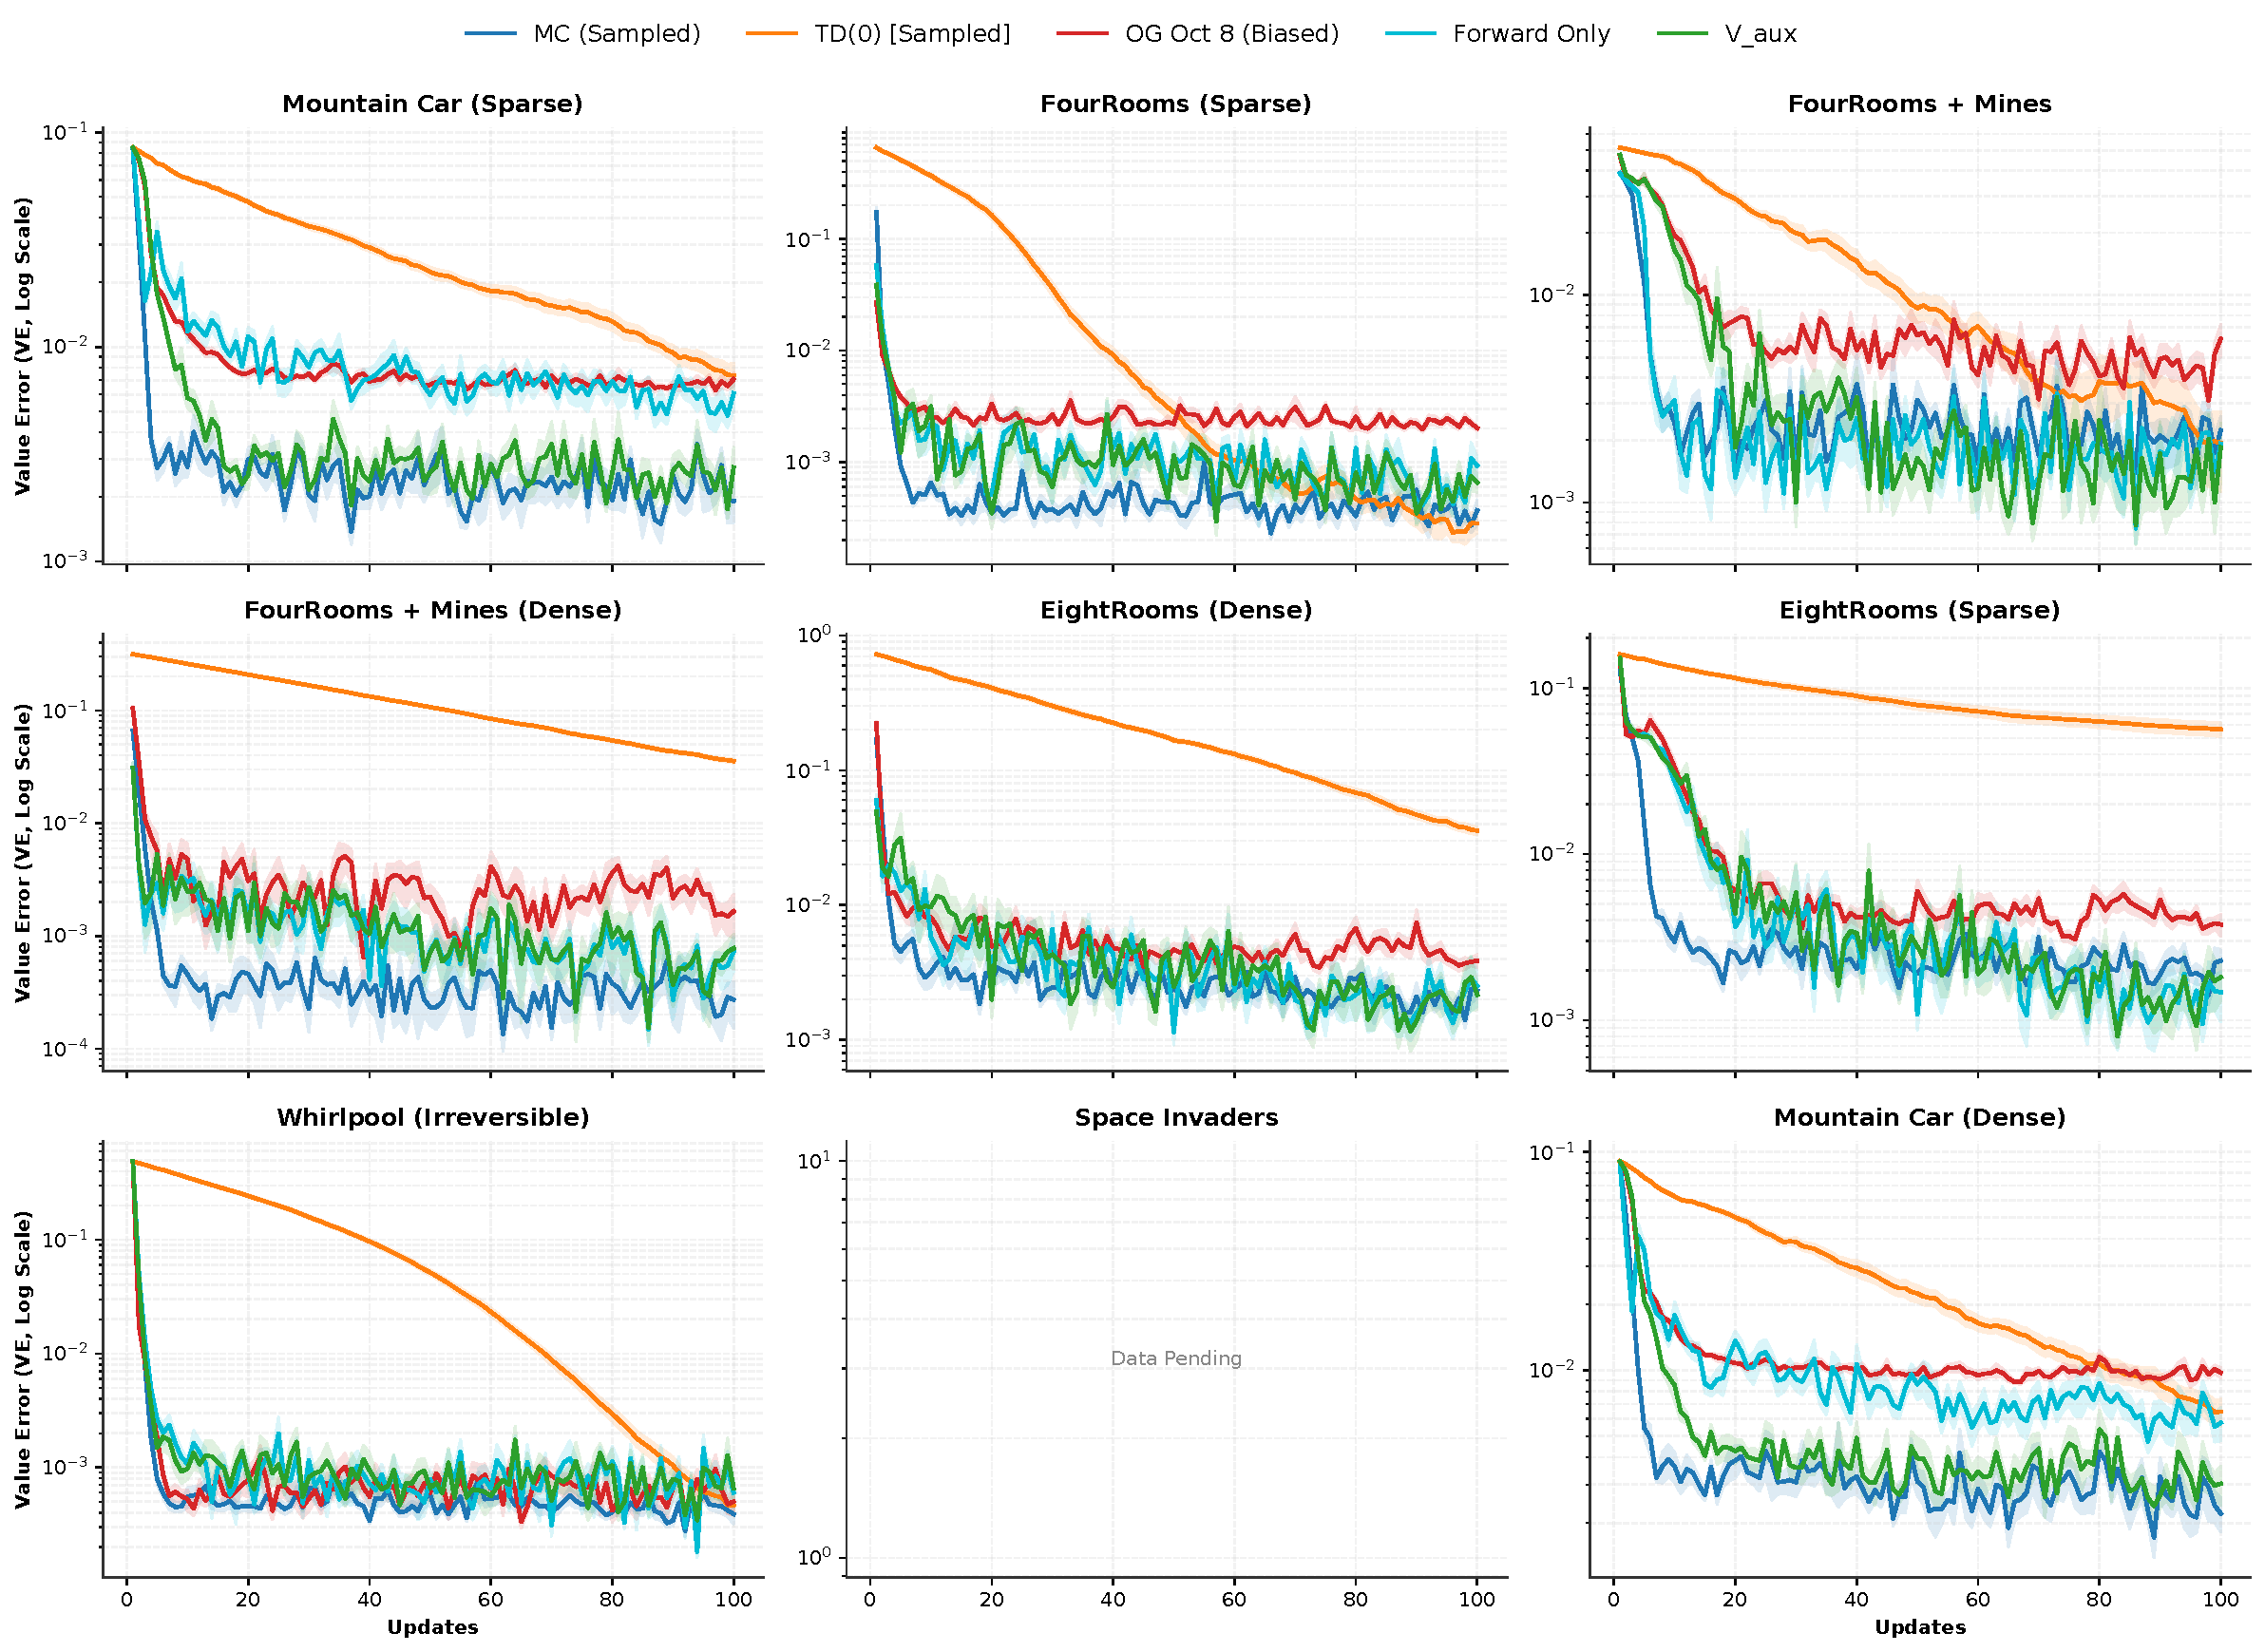
\includegraphics[width=\textwidth]{figures/fixed_pi_ve_curves_all_algos.pdf}
  \caption{\textbf{Value Error in Fixed Policy Evaluation}  10 seeds.}
  \label{fig:fixed_pi_ve_curves_all_algos}
\end{figure*}
% ----------------------------------------------------------------
% End Figure
% ----------------------------------------------------------------

Next, we test these algorithms for control, using them to train the critic in PPO. Observe that Oct 8 does poorly due to the bias in the gradient (although perhaps not as poorly as one might expect given that its value error is an order of magnitude higher). 


% ----------------------------------------------------------------
% Figure: Fixed Pi
% ----------------------------------------------------------------
\begin{figure*}[tbp]
  \centering
  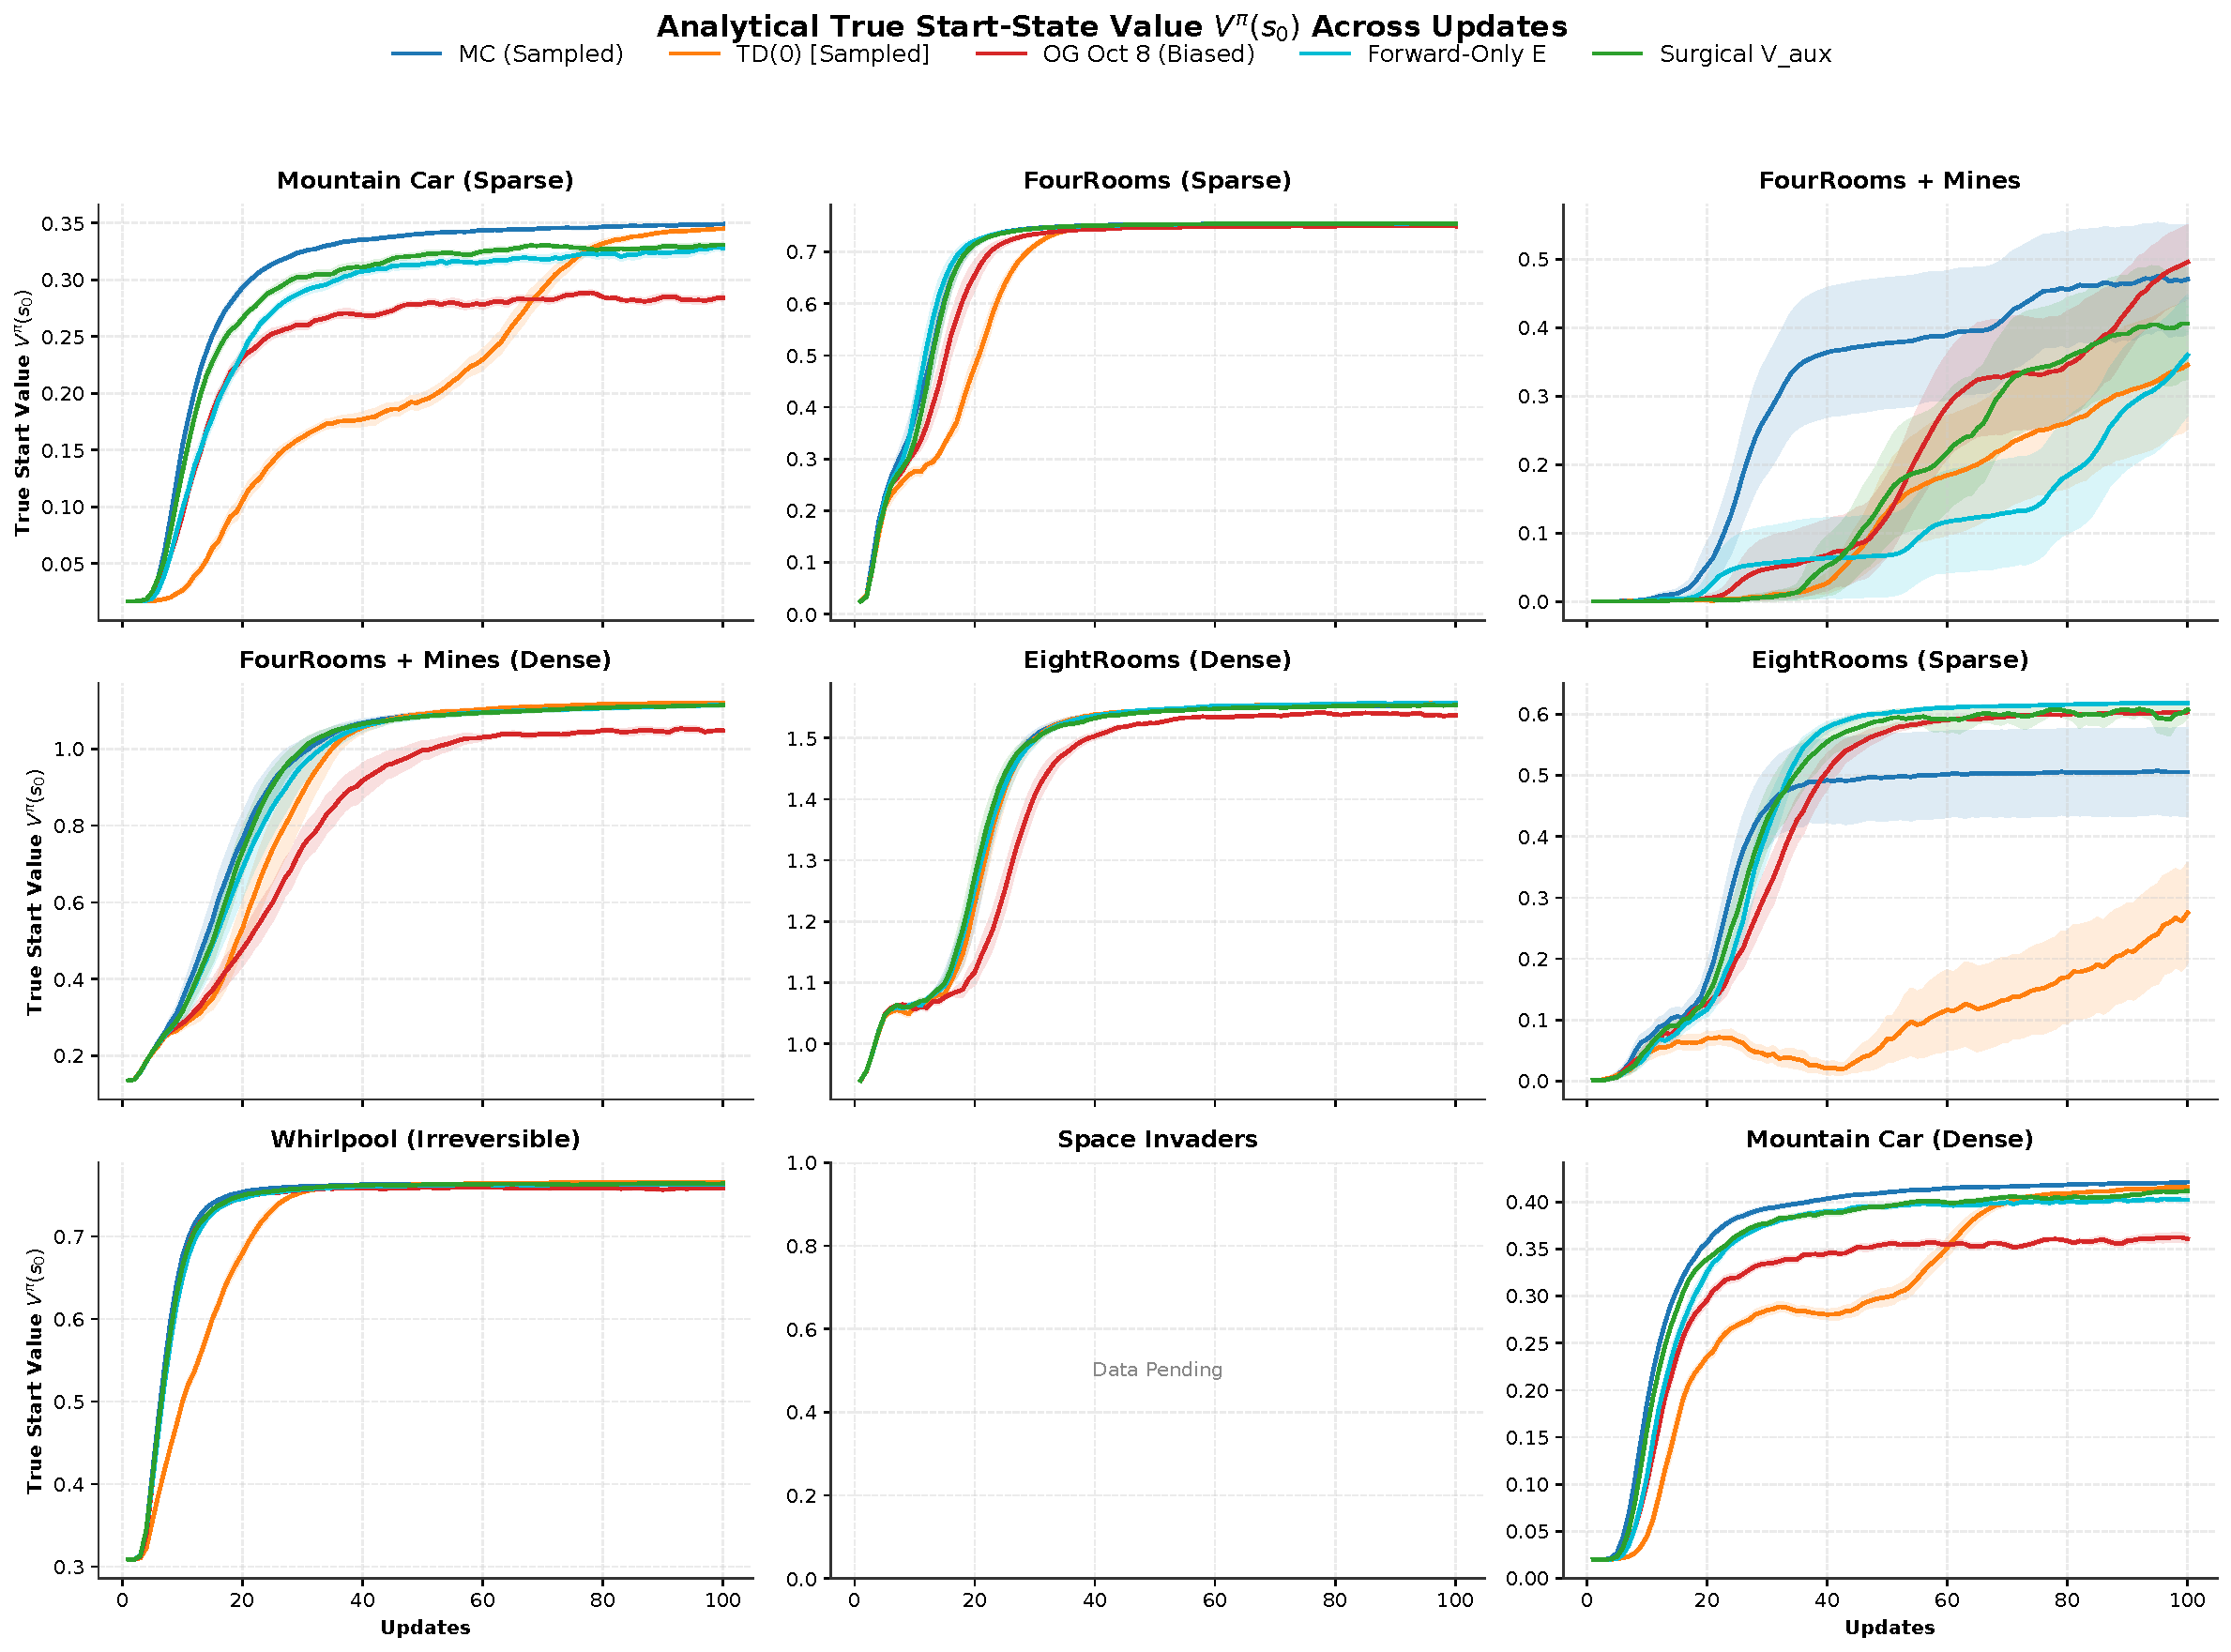
\includegraphics[width=\textwidth]{figures/v_start_curves_all_algos.pdf}
  \caption{\textbf{PPO Performance}: The ground-truth value of the start state is shown, eliminating variance due to measuring returns.  10 seeds.}
  \label{fig:v_start_curves_all_algos}
\end{figure*}
\newpage 
% ----------------------------------------------------------------
% End Figure
% -------------------

% \paragraph{Stochastic Gradient Estimator and Expected Dynamics.}
% Combining the Monte Carlo objective $(1-\gamma)\|e\|_D^2$ with the smoothness energy $\gamma \mathcal{E}$, where Term (1) uses $e_{\text{aux}}(s) \doteq v_{\text{aux}}(s) - v_\theta(s)$ and Term (2) uses the decomposition of Equation~(24), yields the per-transition stochastic gradient estimator $\hat{g}_i$ for transition $(s_i, r_i, s_j)$ and return $G_i^T$:
% \begin{align}
%     \hat{g}_i &= -2(1-\gamma)\hat{e}_i \nabla_\theta v_i 
%     + \gamma \big(e_{\text{aux},i} - e_{\text{aux},j}\big)\nabla_\theta v_j \nonumber \\
%     &\quad - \gamma \big(\hat{\delta}_i - (1-\gamma)\hat{e}_j\big)\nabla_\theta v_i, \label{eq:full_sample_grad}
% \end{align}
% where $v_i \equiv v_\theta(s_i)$, $\hat{\delta}_i = r_i + \gamma v_j - v_i$ is the 1-step TD error, $\hat{e}_i = G_i^T - v_i$, and $\hat{e}_j = G_j^T - v_j$. 
% Crucially, every Monte Carlo return $\hat{e}_i$ and $\hat{e}_j$ is multiplied by $(1-\gamma)$. 
% Since $\mathrm{Var}(G^T) = \mathcal{O}\big((1-\gamma)^{-2}\big)$, scaling by $(1-\gamma)$ yields $\mathrm{Var}\big((1-\gamma)\hat{e}\big) = \mathcal{O}(1)$, independent of the horizon.

% To analyze the expected gradient and fixed point, let $\epsilon_{\text{aux}}(s) \doteq v_{\text{aux}}(s) - V(s)$ denote the auxiliary approximation error, yielding the decomposition $e_{\text{aux}} = e + \epsilon_{\text{aux}}$. 
% Assuming $T$ is sufficiently large that truncation bias is negligible ($\mathbb{E}[\hat{e}_i \mid s_i] = e_i$ and $\mathbb{E}[\hat{\delta}_i \mid s_i] = \delta_i = [(I-\gamma P)e]_i$), taking the expectation over $s_i \sim \mu$ and $s_j \sim P(\cdot \mid s_i)$ gives:
% \begin{align}
%     \mathbb{E}[\hat{g}_i] &= -2(1-\gamma)J_\theta^\top D e + \gamma J_\theta^\top (P^\top - I) D e_{\text{aux}} - \gamma J_\theta^\top D (I - P) e \nonumber \\
%     &= -2 J_\theta^\top \underbrace{\left(D - \frac{\gamma}{2}(DP + P^\top D)\right)}_{S} e + \gamma J_\theta^\top (P^\top - I) D \epsilon_{\text{aux}} \nonumber \\
%     &= \nabla_\theta E + \gamma J_\theta^\top (P^\top - I) D \epsilon_{\text{aux}}. \label{eq:expected_grad_bias}
% \end{align}
% Equation~\eqref{eq:expected_grad_bias} reveals three key properties:
% \begin{enumerate}
%     \item \textbf{Preservation of Symmetric Operator $S$:} Because $e_{\text{aux}}(s_i) - e_{\text{aux}}(s_j)$ contains the exact difference of $v_\theta$, the matrix multiplying $e$ remains the exact symmetric positive-definite matrix $-2 J_\theta^\top S$, retaining stability guarantees regardless of inaccuracies in $v_{\text{aux}}$.
%     \item \textbf{Consistency under Unbiased Auxiliary Regression:} If $v_{\text{aux}}$ converges to the MC regression optimum where $J_\theta^\top D \epsilon_{\text{aux}} = 0$, the bias reduces to $\gamma J_\theta^\top P^\top D \epsilon_{\text{aux}}$, vanishing as $\epsilon_{\text{aux}} \to 0$.
%     \item \textbf{Difference-Filtering of Auxiliary Error:} Because $\epsilon_{\text{aux}}$ is multiplied by $(P^\top - I)D$, any constant offset or smooth error across transitions ($\epsilon_{\text{aux}}(s_i) \approx \epsilon_{\text{aux}}(s_j)$) is automatically cancelled out.
% \end{enumerate}


  \newpage
  \bibliography{main}
  \bibliographystyle{icml2026}
  
  %%%%%%%%%%%%%%%%%%%%%%%%%%%%%%%%%%%%%%%%%%%%%%%%%%%%%%%%%%%%%%%%%%%%%%%%%%%%%%%
  %%%%%%%%%%%%%%%%%%%%%%%%%%%%%%%%%%%%%%%%%%%%%%%%%%%%%%%%%%%%%%%%%%%%%%%%%%%%%%%
  % APPENDIX
  %%%%%%%%%%%%%%%%%%%%%%%%%%%%%%%%%%%%%%%%%%%%%%%%%%%%%%%%%%%%%%%%%%%%%%%%%%%%%%%
  %%%%%%%%%%%%%%%%%%%%%%%%%%%%%%%%%%%%%%%%%%%%%%%%%%%%%%%%%%%%%%%%%%%%%%%%%%%%%%%
  \newpage
  \appendix
  \onecolumn
  
\section{You \emph{can} have an appendix here.}

\textbf{Truncation Bias}
When sampling $E$ using truncated rollouts of length $T$ rather than episodic episodes, 
one can use the $T$-step bootstrapped return, leading to the following approximation of $e_i$ 
\begin{equation}
  G^T_i &= \sum_{t=0}^{T-1} \gamma^t r_t + \gamma^T \overline{v}(s_T) | s_0=s_i \\
  e_i &\approx \delta^T_i &= G^T_i - \overline{v}(s_i) \label{eq:approxewithdelta}
\end{equation}

The quality of the approximation in Equation \ref{eq:approxewithdelta} improves with $T$, becoming exact as $T \rightarrow \infty$. 

We call the bias in estimating the the Bellman Smoothed Value Error with $\delta^T_i$ instead of $e_i$ \textit{truncation bias}. Using the Generalized Advantage Estimation (GAE) with $\lambda=1$ on fixed-length rollouts will result in truncation bias increasing with the position in the rollout, finally resulting in $e_T$ being approximated by $\delta_t$. Examining the energy for this final transition:

\begin{align}
  \mathcal{E}_T &\approx \frac{1}{2} (G_T - v(s_T) - G_{T+1} + v(s_{T+1}) )^2 \\
  &\approx \frac{1}{2} (r_T + \gamma \overline v(s_{T+1}) - v(s_T) - (v(s_{T+1}) - v(s_{T+1}) ))^2 \\
  &\approx \frac{1}{2} (r_T + \gamma \overline v(s_{T+1}) - v(s_T))^2
\end{align}

That is, the estimate of $E$ obtained at the final step in the batch reverts to $\mathcal{L}_{TD}$. 

\textbf{Experiment: Truncation Bias}
We examine how truncation bias scales on small environments. We run PPO on each environment. PPO's update step first collects $B$ parallel trajectories of length $T$, and then updates the actor and critic for a number of gradient steps. At each update step, we compute the expectation of the gradient $\bm{g}^* = \mathbb{E}_\mu \nabla_\theta E$, and the estimate on the sampled data $\hat{\bm{g}} = \frac{1}{TB}\sum_{b=1}^B \sum_{t=1}^T \nabla_\theta l_e(s_{b,t}, s_{b,t+1}, G^T_{b,t}, G^T_{b, t+1})$. Both $\hat{\bm{g}}$ and $\bm{g}^*$ are length $k$ vectors in paramter space. The MSE $\|\hat{\bm{g}} - \bm{g}^*\|_2^2$ is the sum of the squared truncation bias and variance.

% ------------------------------------------------------------------------------
% Figure: Performance on Tasks with T
% ------------------------------------------------------------------------------
\begin{figure*}[ht]
  \centering
  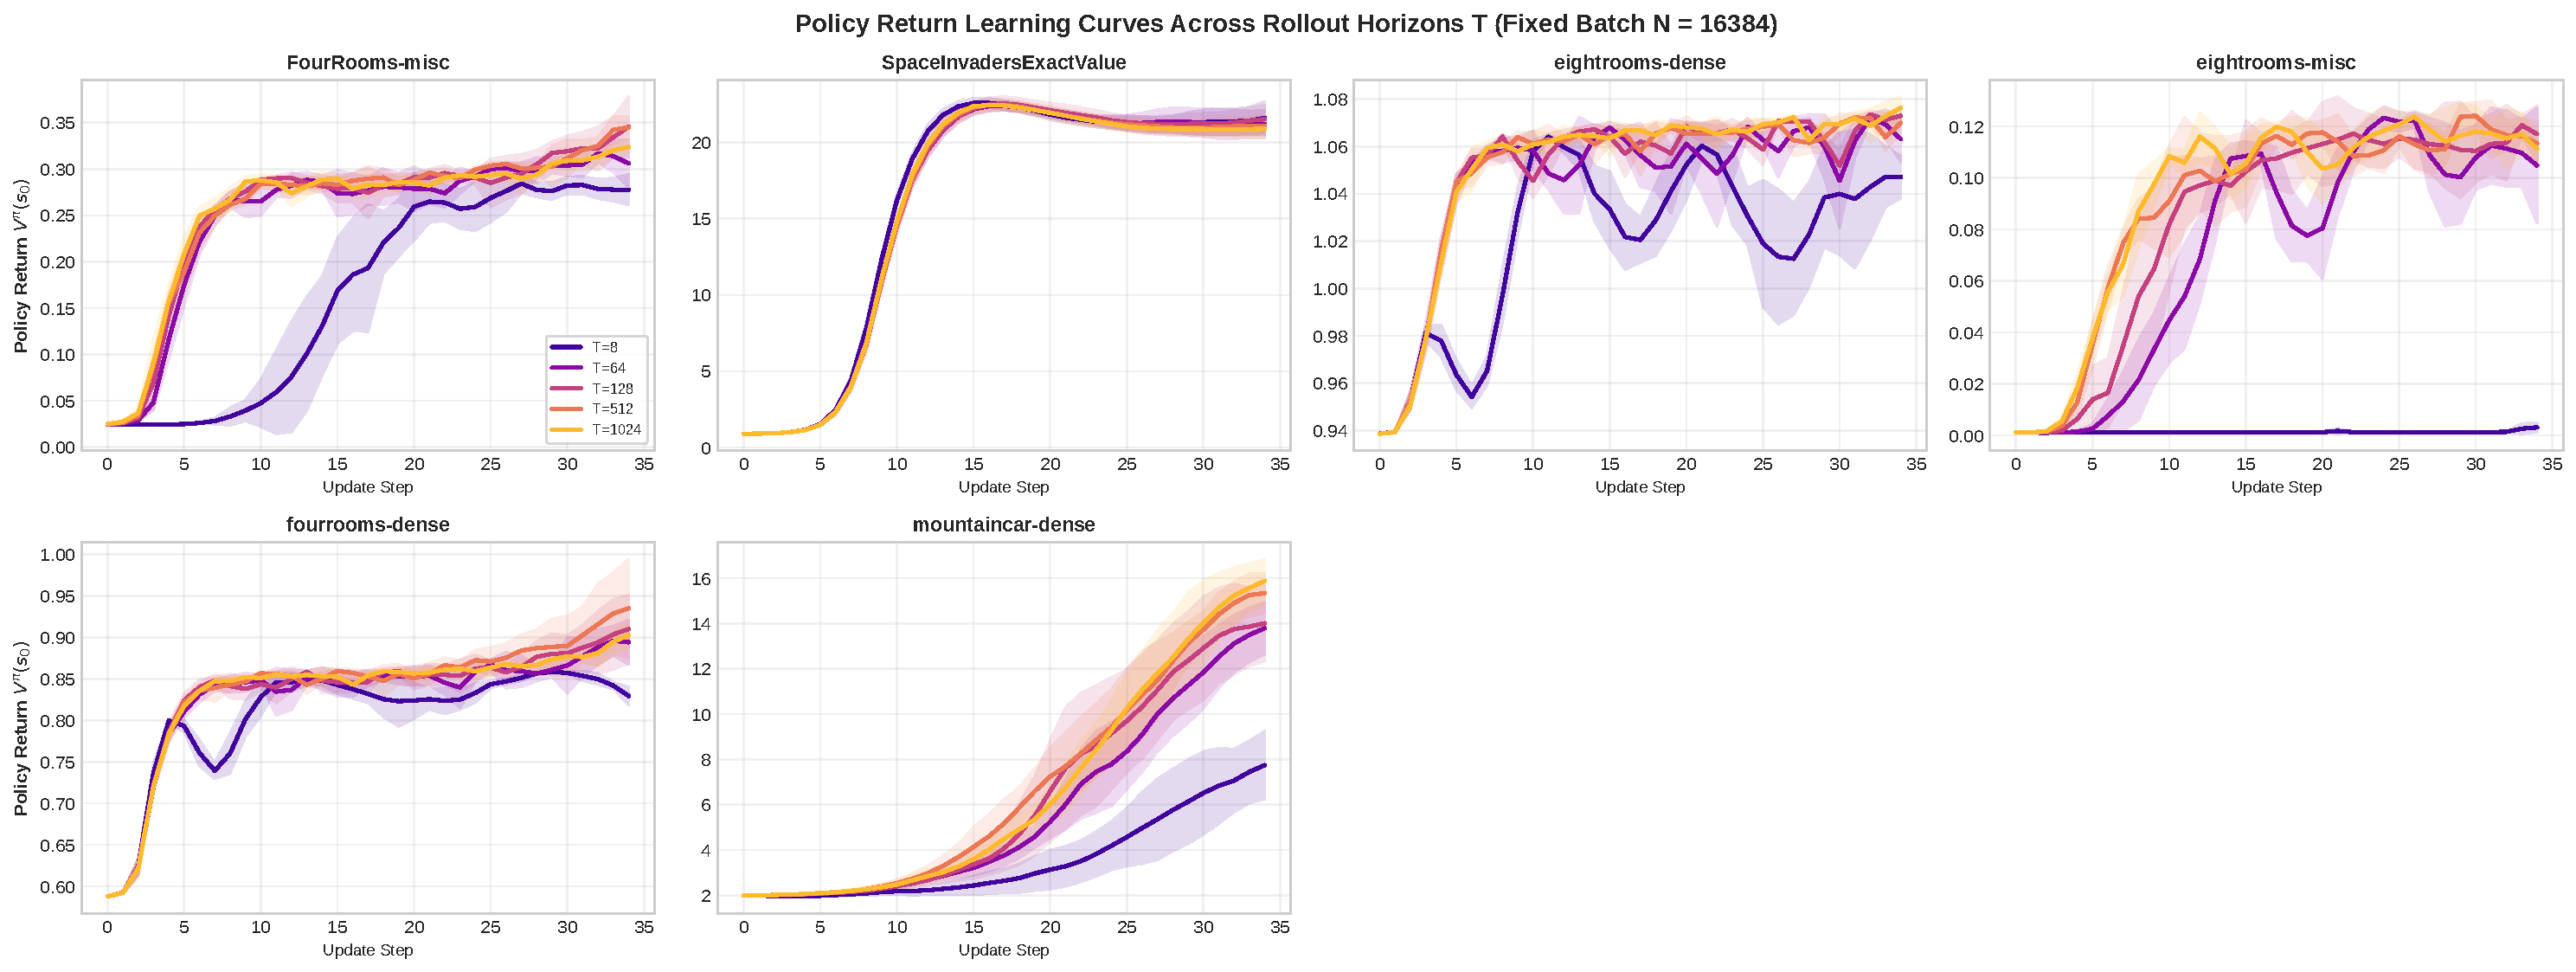
\includegraphics[width=\textwidth]{figures/cross_env_policy_returns_all_T.pdf}
  \caption{\textbf{Performance of PPO using E-Based Critic by Horizon} 
  Performance of PPO with value learning due to the (sampled) Bellman Smoothed Value Loss for different horizon values $T$. Each horizon still has the same number of samples and gradient steps per update.}
  \label{fig:small_ppo_performance_by_T}
\end{figure*}
% ------------------------------------------------------------------------------
% End Figure
% ------------------------

Figure \ref{fig:small_ppo_performance_by_T} shows performance during learning for each considered rollout length $T$, demonstrating that performance generally improved with $T$. 

Figure \ref{fig:squared_error_trajectories} shows estimated $\text{Bias}^2$ and Variance, finding that generally the bias decreases with $T$, while variance increases. 

Figure \ref{fig:squared_error_trajectories} shows the mean squared error of the gradient $\|\hat{\bm{g}} - \bm{g}^*\|_2^2$ during learning. 

% Figure \ref{fig:final_return_vs_T} shows final performance as a function of $T$.
------------------------------------------------------

% ------------------------------------------------------------------------------
% Figure 1: Main Bias-Variance Decomposition across Horizons T
% ------------------------------------------------------------------------------
\begin{figure*}[ht]
  \centering
  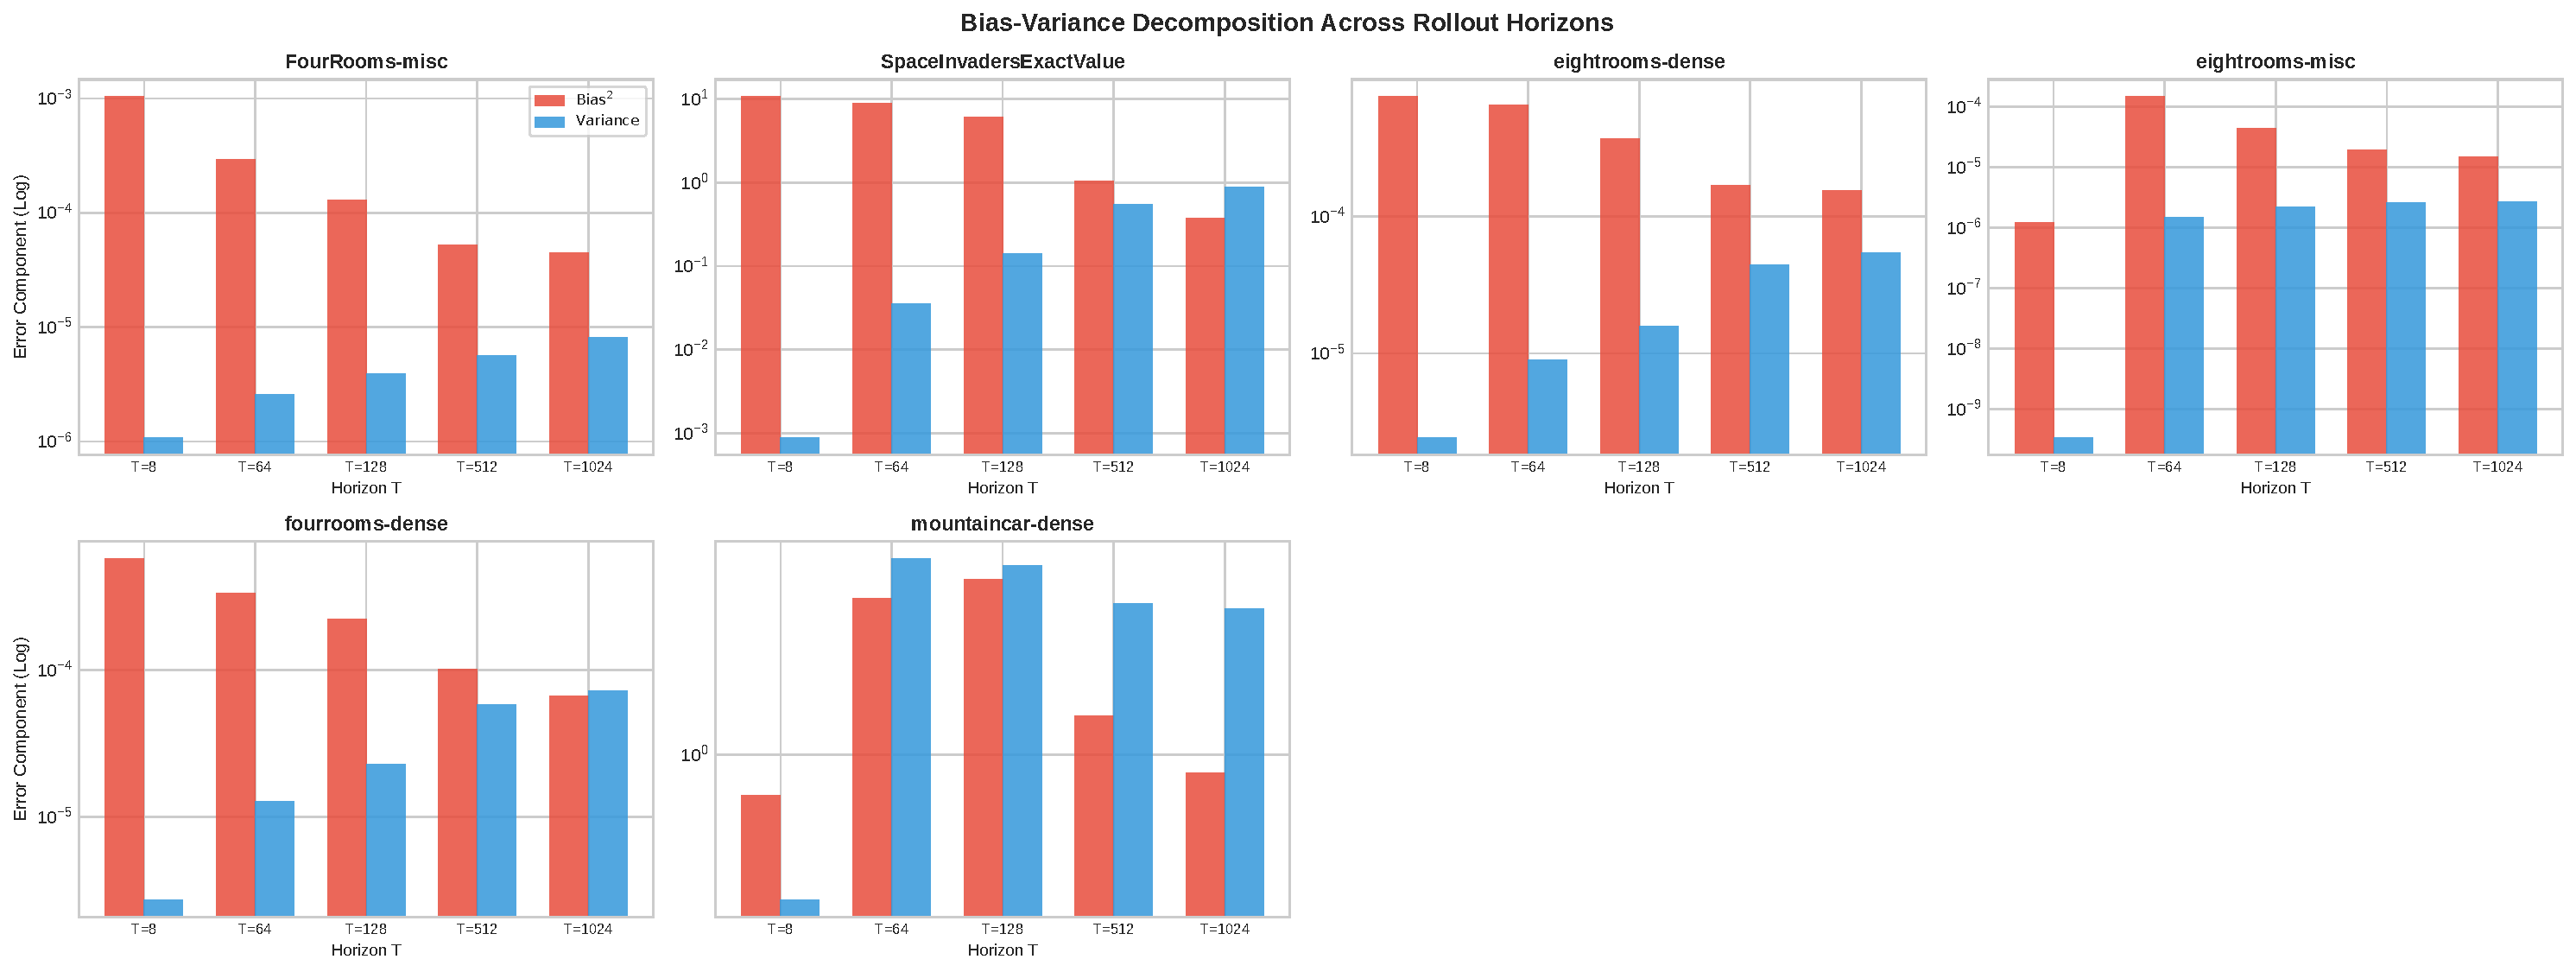
\includegraphics[width=\textwidth]{figures/cross_env_bias_variance_summary.pdf}
  \caption{\textbf{Bias-Variance Trade-off in Bellman Error Gradient Estimation ($N = B \times T = 16{,}384$).} 
  Decomposition of the total gradient mean squared error $\|\hat{\bm{g}} - \bm{g}^*\|_2^2 = \text{Bias}^2 + \text{Variance}$ across rollout horizons $T \in \{8, 64, 128, 512, 1024\}$. As the rollout horizon $T$ increases, truncation bias strictly decreases as the $T$-step return approximation $\delta_i^T \to e_i$ becomes exact. Concurrently, sample variance increases due to the reduced number of parallel trajectory rollouts $B = N / T$ under a fixed computational budget. Note that there is bias in the estimate of $\text{Bias}^2$ itself, preventing it from going to zero.}
  \label{fig:truncation_bias_variance}
\end{figure*}
% ------------------------------------------------------------------------------
% End Figure
% ------------------------------------------------------------------------------
% ------------------------------------------------------------------------------
% Figure 2: Learning Curves (Gradient MSE Trajectories & Final Return vs T)
% ------------------------------------------------------------------------------
\begin{figure*}[t]
  \centering
  % Top panel: Full page width
  \begin{subfigure}[b]{\textwidth}
    \centering
    \includegraphics[width=\textwidth]{figures/cross_env_squared_error_trajectories.pdf}
    \caption{Gradient Squared Error $\|\hat{\bm{g}} - \bm{g}^*\|_2^2$ Across Learning Updates (Log Scale)}
    \label{fig:squared_error_trajectories}
  \end{subfigure}
  
  \vspace{0.8em} % Spacing between panels
  
  % Bottom panel: Full page width
  \begin{subfigure}[b]{\textwidth}
    \centering
    \includegraphics[width=\textwidth]{figures/cross_env_final_return_vs_T.pdf}
    \caption{Asymptotic Policy Performance $V^\pi(s_0)$ as a Function of Rollout Horizon $T$}
    \label{fig:final_return_vs_T}
  \end{subfigure}
  
  \caption{\textbf{Gradient Error and Policy Performance by Rollout Length.} 
  \textbf{(a)} The empirical gradient MSE $\|\hat{\bm{g}} - \bm{g}^*\|_2^2$ over policy updates across 7 environments. Shorter horizons suffer from persistent truncation bias floors, while longer horizons ($T \ge 512$) drive gradient error orders of magnitude lower. 
  \textbf{(b)} Final policy return $V^\pi(s_0)$ vs. horizon $T$, demonstrating that reducing truncation bias usually improves downstream policy optimization.}
  \label{fig:error_and_return_curves}
\end{figure*}
% ------------------------------------------------------------------------------
% End Figure
% ------------------------------------------------------------------------------


\section{Deep RL Experiments}

\begin{figure*}[ht]
  \centering
  \includegraphics[width=\textwidth]{figures/td0_vs_e_gymnax.pdf}
  \caption{\textbf{Gymnax TD(0) vs E(0).} 
  Decomposition of the total gradient mean squared error $\|\hat{\bm{g}} - \bm{g}^*\|_2^2 = \text{Bias}^2 + \text{Variance}$ across rollout horizons $T \in \{8, 64, 128, 512, 1024\}$. As the rollout horizon $T$ increases, truncation bias strictly decreases as the $T$-step return approximation $\delta_i^T \to e_i$ becomes exact. Concurrently, sample variance increases due to the reduced number of parallel trajectory rollouts $B = N / T$ under a fixed computational budget. Note that there is bias in the estimate of $\text{Bias}^2$ itself, preventing it from going to zero.}
  \label{fig:gymnaxetd}
\end{figure*}





\subsection*{Bias-Variance Decomposition of Gradient Estimates}

Let $\bm{g}^* = \mathbb{E}_{\mu^\pi}[\nabla_\theta \mathcal{E}]$ denote the exact expected Bellman error gradient in parameter space $\mathbb{R}^k$, and let $\hat{\bm{g}} \in \mathbb{R}^k$ denote the empirical gradient computed from a batch of $B$ rollout trajectories of horizon $T$. 

\subsubsection*{1. Population Bias-Variance Decomposition}
Defining the population expectation of the sampled gradient as $\bm{\mu}_{\hat{\bm{g}}} \triangleq \mathbb{E}[\hat{\bm{g}}]$, the total Mean Squared Error (MSE) decomposes into the squared truncation bias and the trace of the gradient covariance matrix:
\begin{align}
  \mathrm{MSE}(\hat{\bm{g}}) 
  &\triangleq \mathbb{E}\left[ \|\hat{\bm{g}} - \bm{g}^*\|_2^2 \right] \nonumber \\
  &= \mathbb{E}\left[ \|\left(\hat{\bm{g}} - \bm{\mu}_{\hat{\bm{g}}}\right) + \left(\bm{\mu}_{\hat{\bm{g}}} - \bm{g}^*\right)\|_2^2 \right] \nonumber \\
  &= \|\bm{\mu}_{\hat{\bm{g}}} - \bm{g}^*\|_2^2 
     + \mathbb{E}\left[ \|\hat{\bm{g}} - \bm{\mu}_{\hat{\bm{g}}}\|_2^2 \right] 
     + 2\,\underbrace{\mathbb{E}\left[\hat{\bm{g}} - \bm{\mu}_{\hat{\bm{g}}}\right]^\top}_{=\,\bm{0}} \left(\bm{\mu}_{\hat{\bm{g}}} - \bm{g}^*\right) \nonumber \\
  &= \underbrace{\|\bm{\mu}_{\hat{\bm{g}}} - \bm{g}^*\|_2^2}_{\text{Truncation Bias}^2} 
     + \underbrace{\vphantom{\|\bm{\mu}_{\hat{\bm{g}}} - \bm{g}^*\|_2^2} \operatorname{Tr}\left(\operatorname{Cov}(\hat{\bm{g}})\right)}_{\text{Sample Variance}}. \label{eq:pop_bias_var}
\end{align}

\subsubsection*{2. Empirical Sample-Level Decomposition}
In empirical experiments, we evaluate $M$ independent stochastic runs (seeds) $\{\hat{\bm{g}}^{(m)}\}_{m=1}^M$ under identical policy parameters, and compute the sample mean gradient:
\begin{equation}
  \bar{\bm{g}} = \frac{1}{M} \sum_{m=1}^M \hat{\bm{g}}^{(m)}.
\end{equation}
By Huygens' sum-of-squares identity, the total empirical MSE partitions exactly into two non-negative terms:
\begin{align}
  \underbrace{\frac{1}{M} \sum_{m=1}^M \|\hat{\bm{g}}^{(m)} - \bm{g}^*\|_2^2}_{\widehat{\mathrm{MSE}}} 
  &= \underbrace{\|\bar{\bm{g}} - \bm{g}^*\|_2^2}_{\widehat{\mathrm{Bias}}^2_{\mathrm{sample}}} 
   + \underbrace{\frac{1}{M} \sum_{m=1}^M \|\hat{\bm{g}}^{(m)} - \bar{\bm{g}}\|_2^2}_{\widehat{\mathrm{Var}}_{\mathrm{sample}}}. \label{eq:sample_bias_var}
\end{align}
This algebraic identity guarantees that $\widehat{\mathrm{MSE}} \equiv \widehat{\mathrm{Bias}}^2_{\mathrm{sample}} + \widehat{\mathrm{Var}}_{\mathrm{sample}}$ strictly holds across all seeds and horizons without leaving an unassigned residual or generating negative quantities on logarithmic plots.

\subsubsection*{3. Finite-Sample Expectation of the Estimator}
Taking the expectation of the empirical plug-in bias estimator $\widehat{\mathrm{Bias}}^2_{\mathrm{sample}}$ reveals that it is a biased estimator of the true population squared bias $\|\bm{\mu}_{\hat{\bm{g}}} - \bm{g}^*\|_2^2$:
\begin{align}
  \mathbb{E}\left[ \widehat{\mathrm{Bias}}^2_{\mathrm{sample}} \right] 
  &= \mathbb{E}\left[ \|\bar{\bm{g}} - \bm{g}^*\|_2^2 \right] \nonumber \\
  &= \mathbb{E}\left[ \|\left(\bar{\bm{g}} - \bm{\mu}_{\hat{\bm{g}}}\right) + \left(\bm{\mu}_{\hat{\bm{g}}} - \bm{g}^*\right)\|_2^2 \right] \nonumber \\
  &= \|\bm{\mu}_{\hat{\bm{g}}} - \bm{g}^*\|_2^2 + \mathbb{E}\left[ \|\bar{\bm{g}} - \bm{\mu}_{\hat{\bm{g}}}\|_2^2 \right] \nonumber \\
  &= \|\text{Bias}(\hat{\bm{g}})\|_2^2 + \frac{1}{M} \operatorname{Tr}\left(\operatorname{Cov}(\hat{\bm{g}})\right). \label{eq:bias_floor}
\end{align}
Consequently, due to the convexity of the $L_2$ norm (Jensen's inequality), $\widehat{\mathrm{Bias}}^2_{\mathrm{sample}}$ carries an unavoidable additive variance penalty of $\frac{1}{M}\mathrm{Var}(\hat{\bm{g}})$. Even in the asymptotic limit where truncation bias vanishes ($\bm{\mu}_{\hat{\bm{g}}} \to \bm{g}^*$ as $T \to \infty$), the empirical sample bias hits a noise floor of $\frac{1}{M}\mathrm{Var}(\hat{\bm{g}}) > 0$.

An unbiased estimator of population squared bias is given by:
\begin{equation}
  \widehat{\mathrm{Bias}}^2_{\mathrm{unbiased}} = \|\bar{\bm{g}} - \bm{g}^*\|_2^2 - \frac{1}{M-1}\widehat{\mathrm{Var}}_{\mathrm{sample}},
\end{equation}
which subtracts the finite-sample variance penalty at the expense of potentially admitting negative values under finite sample noise when the true bias is negligible.


You can have as much text here as you want. The main body must be at most $8$
pages long. For the final version, one more page can be added. If you want, you
can use an appendix like this one.

The $\mathtt{\backslash onecolumn}$ command above can be kept in place if you
prefer a one-column appendix, or can be removed if you prefer a two-column
appendix.  Apart from this possible change, the style (font size, spacing,
margins, page numbering, etc.) should be kept the same as the main body.
%%%%%%%%%%%%%%%%%%%%%%%%%%%%%%%%%%%%%%%%%%%%%%%%%%%%%%%%%%%%%%%%%%%%%%%%%%%%%%%
%%%%%%%%%%%%%%%%%%%%%%%%%%%%%%%%%%%%%%%%%%%%%%%%%%%%%%%%%%%%%%%%%%%%%%%%%%%%%%%

\end{document}

% This document was modified from the file originally made available by
% Pat Langley and Andrea Danyluk for ICML-2K. This version was created
% by Iain Murray in 2018, and modified by Alexandre Bouchard in
% 2019 and 2021 and by Csaba Szepesvari, Gang Niu and Sivan Sabato in 2022.
% Modified again in 2023 and 2024 by Sivan Sabato and Jonathan Scarlett.
% Previous contributors include Dan Roy, Lise Getoor and Tobias
% Scheffer, which was slightly modified from the 2010 version by
% Thorsten Joachims & Johannes Fuernkranz, slightly modified from the
% 2009 version by Kiri Wagstaff and Sam Roweis's 2008 version, which is
% slightly modified from Prasad Tadepalli's 2007 version which is a
% lightly changed version of the previous year's version by Andrew
% Moore, which was in turn edited from those of Kristian Kersting and
% Codrina Lauth. Alex Smola contributed to the algorithmic style files.

